\documentclass[format=acmlarge, review=false, nonacm=false, screen=true]{acmart}

\settopmatter{printacmref=false}
\renewcommand\footnotetextcopyrightpermission[1]{}
\pagestyle{plain}
\setcopyright{none}

\usepackage{soul}
\usepackage{hyperref}
\usepackage{minted}
\usepackage[utf8]{inputenc}
\graphicspath{ {./figures/} }
\makeatletter
\AtBeginEnvironment{minted}{\dontdofcolorbox}
\def\dontdofcolorbox{\renewcommand\fcolorbox[4][]{##4}}
\makeatother

\begin{document}
\title{Background Report:\\Visualizing the FWAE Language}

\author{Megha Singhania}
\affiliation{t4u0b@ugrad.cs.ubc.ca}
\author{Jonathan Chan}
\affiliation{r5x9a@ugrad.cs.ubc.ca}
\author{Samuel Or}
\affiliation{u4h1b, or.samuel1@gmail.com}
\author{Xuhao Chen}
\affiliation{d4i0b@ugrad.cs.ubc.ca}

\begin{abstract}
\vspace{1em}

Our project is of the fourth type: to create a substantial program in an esoteric language. It strives to produce an educational tool for the CPSC 311 course by providing parse tree and call tree visualizations, complete with environment and state illustrations, for the FWAE course language, which includes first-class functions but not mutation (e.g. \texttt{box} features), laziness, or explicit recursive constructs (e.g. \texttt{rec-with} and \texttt{rec-apply}). The parser and visualizer will both be implemented using Haskell, making use of the lazy and functional features of the language, as well as well-known libraries for parsing and visualization.
\end{abstract}

\maketitle

\setcounter{section}{-1}
\section{Introduction}
\subsection{Motivation}
\textbf{Functions are powerful.} As was stated in CPSC 311, once a language has first-class functions and function application, that language is now as powerful as any other in terms of computational ability. All other features covered in CPSC 311, such as mutation, recursion, and laziness, are all built upon the framework of a parser and interpreter that implements first-class functions. It is therefore crucial that any student of CPSC 311 fully understand this basic implementation and have a correct mental model before moving on to more complex ideas.

Very often, mental models are based not in words or concrete code but in visual diagrams. This is illustrated, quite literally, by how often the CPSC 311 professor will use the whiteboard to draw parse trees and call trees early in the course to explain what is to be implemented in code. This is naturally both time-consuming and error-prone, as human activities often are. It is for this reason that we will implement a parse tree and call tree visualizer to automate the process, and we hope that our tool will bring great benefit not only to students but also instructors of CPSC 311.

\begin{comment}
Because half of the tools would revolve around parsing the first-class language FWAE, the language we use should be well-suited to parsing. Among many, there are two notable choices: Racket, for its built-in ability to transform LISP-like statements into lists, and Haskell, in which is implemented a common parsing library called Parsec, making use of abstracted functional concepts called monadic parser combinators. We have chosen the latter, not only to satisfy project requirements, but also ???
\end{comment}

\subsection{Goals}
The remainder of this report is divided into three sections. In the first section, we will discuss various important features of Haskell, such as data types, built-in language constructs, and laziness, that we will make use of in the project. This will be followed by a section on parsing and how we will use the Parsec library to parse one of the course languages implemented in CPSC 311, FWAE, which will be part of our 90\%-level goal. Finally, in the last section, we will outline a basic usage of ghc-vis to create interactive visualizations of our abstract syntax tree and of a call tree resulting from interpretation, which would be included in the 100\%-level goal. For this project, we are aiming for the 90\%-level.

\section{A Primer on Haskell}
Haskell is a purely functional programming language, which means that code is not written as a sequence of tasks for the computer to execute, like the languages we are more used to such as Python, C, and Java. A benefit of pure functional languages is that no side-effects can occur in a function, and they just simply return a result. This generally allows for more clean and compact code compared to its imperative style counterpart. In the following subsections, we will discuss certain features that distinguish Haskell from other languages.

\subsection{Type Inference}

One unique feature of Haskell is its type inference. Haskell determines the type of every expression at compile time. For example, in Java, the syntax for declaring a variable is:
\begin{minted}{java}
int n = 5;
\end{minted}
Java requires the programmer to declare the type of variable before the name, in this case \texttt{int}, whereas in Haskell all that is required is \texttt{n = 5}, and the compiler infer that \texttt{n} is an integer. By allowing type annotations to be optional most of the time, it provides the benefit of static type-checking without the verbosity that other non--type-inferring languages usually have.

\subsection{Data Types and Pattern-Matching}
In Haskell, data types are data structures that strongly resemble those of Racket's PLAI package. What are called variants are instead called data constructors, since they are functions that construct a particular variant. For instance, if we have the following Racket define-type:

\begin{minted}{racket}
(define-type FAE    
  [num (n number?)] 
  [add (lhs FAE?) (rhs FAE?)])
\end{minted}

This is equivalent to the following Haskell data type:

\begin{minted}{haskell}
data FAE = Num Double
         | Add FAE FAE
zero = Num 0
addOneTwoExpr = Add 1 2
\end{minted}

Rather than using contract expressions, Haskell directly enforces the types of the constituents of each variant. Note that in Haskell, data types and data constructors must begin with a capital letter. Notice also that the parameter names of each variant are missing. This is because in Haskell, no accessor and setter methods are automatically generated, as would be with PLAI; instead, we can directly pattern-match to the structure of variant. As a concrete example, the following is a function that returns true if given a number, and false if given an addition expression.

\begin{minted}{haskell}
isNumber :: FAE -> Boolean
isNumber (Num n)       = True
isNumber (Add lhs rhs) = False
\end{minted}

Using pattern-matching means we essentially redefine a function for every pattern we wish to match to, explicitly deconstructing the data structure on the left side of the function declaration. In the above, the \texttt{Double} stored in the \texttt{Num} is bound to \texttt{n}, while the two \texttt{FAE} expressions stored in the \texttt{Add} are bound to \texttt{lhs} and \texttt{rhs}, respectively.

\begin{comment}
\subsection{Useful Language Constructs}
Since we need to construct a parser for the FWAE language for this project, a significant section of the project would rely on reading a certain sequence of expressions and spitting out another, also known as pattern matching. Haskell allows us to simply do this by writing a function that, for example, takes a \texttt{String} and returns a \texttt{String}. The reason why writing this function is so simple is because of Haskell's syntax. If you wanted to write a switch statement, each case can be done in one line: `function name' `case' = `result'. This can also be applied to arrays as well. Haskell also has an interesting syntax that simplifies reading else-if clauses, which are called guards. Guards look like this:
\begin{minted}{haskell}
f i =
    | i < 10 ten = "less than 10"
    | i < 100 hundred = "less than 100"
    | i < 1000 thousand = "less than 1000"
    | otherwise = "that's a big number"
\end{minted}
Every line above would representing moving deeper into a nested else-if clause, but as shown above, guards makes these nested else-if clauses much more readable, and easier to write as well.
\end{comment}

\begin{comment}
\subsection{Type Constructors and Typeclasses}\label{typeclasses}
In Haskell, types themselves can be functions that take in other types to produce a type. For instance, the \texttt{List} type is commonly defined as follow:

\begin{minted}{haskell}
data List a = Cons a (List a) | Empty
\end{minted}

Then the type of a list of strings would be \texttt{List String}. This implies that the non-trivial constructor of the list of strings is \texttt{Cons String (List String)}, i.e. that we cons a string onto a list of strings. (This also implies that Haskell lists are homogenous.)
\end{comment}

\subsection{Intergrating Laziness}
Haskell evaluates a program using lazy evaluation, which means the evaluation of expressions are deferred until the results are needed for other computations. This feature is helpful to increase performance by avoiding needless visualization of a FWAE tree. The evaluation of expressions inside can be delayed if it is not needed by the outer expression. For this project, it is possible to combine the lazy evaluation with memoization. Some trivial results of interpretation can be stored in a look-up table to be looked up if same interpreter output is encountered.

\section{Parser Combinators and Parsec}
For the 90\% level, we will implement an FWAE parser in Haskell using Parsec, a monadic parser combinator library \cite{parsec}. The following few sections will describe what monadic parsers are and how we will build up to using them, while sections~\ref{gentokenparser} and onwards will describe specific features of Parsec.
\subsection{FAE: An Abstract Syntax Data Type}
The version of FWAE we will be parsing is defined by the following EBNF, taken from the final version of the in-class notes for lecture 6 \cite{inclass6}, with the addition of branching.
\begin{minted}{ebnf}
<FWAE> :: <num>
        | <id>
        | {<op> <FWAE> <FWAE>}
        | {if0 <FWAE> <FWAE> <FWAE>}
        | {fun {<id>} <FWAE>}
        | {<FWAE> <FWAE>}
        | {with {<id> <FWAE>} <FWAE>}
<op>   :: + | - | *
<id>   :: (* begins with letter, rest are alphanumeric or `-` or `_` or `*` *)
          (* is none of `with`, `fun`, `if0`, `+`, `-`, `*` *)
\end{minted}
These translate quite directly into abstract syntax with Haskell's data types:
\begin{minted}{haskell}
data FAE = Number Double
         | Id     String
         | Op     OpType FAE FAE
         | If0    FAE FAE FAE
         | Fun    String FAE
         | App    FAE FAE
    deriving (Show, Eq)
data OpType = Add | Sub | Mul deriving (Show, Eq)
\end{minted}
They derive \texttt{Show} and \texttt{Eq} in order to be printable when interpreting in the REPL and equatable when doing testing. The restrictions on \texttt{<id>} will be enforced by built-in parsers during parsing; for now, they are simply strings, as Haskell does not have built-in symbols like Racket.
We can also define value and environment data types pretty much identically to their Racket PLAI counterparts:
\begin{minted}{haskell}
data Value  = NumV Double | ClosureV String FAE Env deriving (Show, Eq)
data Env    = MtEnv | AnEnv String Value Env deriving (Show, Eq)
\end{minted}
Notice that all numbers are of type \texttt{Double}. Retricting the contained number to being only of typeclass \texttt{Num} would require creating some complex GADTs and interfere with the automatic deriving of \texttt{Show}, so during parsing we will cast all numbers to floating-point numbers.

Since we also want to create a visualization of the call tree, we need a corresponding data structure. Obviously it will be based on \texttt{FAE}, but with the addition of a metadata value that stores the environment and the evaluated value at each point, and with the following changes:
    \begin{itemize}
        \item We will remove terminal values from each variant, since they are no longer relevant to the call tree, and their data would be encapsulated in the return values held in the metadata;
        \item \texttt{If0} will lose a subexpression, since it executes only one of its branches; 
        \item \texttt{Fun} will lose its only subexpression, since the function body is not called at declaration; and
        \item \texttt{App} will gain a subexpression, corresponding to the delayed call of its function's body.
    \end{itemize}
It might then look something like this:
\begin{minted}{haskell}
data CallTree = NumberTree Metadata
              | IdTree     Metadata
              | OpTree     Metadata CallTree CallTree          -- lhs rhs
              | If0Tree    Metadata CallTree CallTree          -- cond on0/non0
              | FunTree    Metadata
              | AppTree    Metadata CallTree CallTree CallTree -- fun arg app
    deriving (Show, Eq)
type Metadata = (Value, Env)
\end{minted}

\subsection{Monadic Parsers}
As mentioned, Monad is a class of data structures that implement certain monadic functions and follow certain monadic laws. For our purposes, it suffices to think of a monadic parser as a wrapper around a parse result that we need to extract. This allows us to abstract away from how the parser consumes and interacts with the input string, and focus on the high-level sequence of actions we want to perform on it. Haskell has many operators that allow us to do this very concisely, and the relevant few are as follows, with an imaginary \texttt{Parser a} type that denotes a parser returning some value of type \texttt{a}:
    \begin{itemize}
        \item \texttt{return :: a -> Parser a}: Wraps a given value in a parser, doing nothing to the input string.
        \item \texttt{>>= :: Parser a -> (a -> Parser b) -> Parser b}: Returns a parser that executes the given parser, applies the given function to the value extracted from that parser, and returns the parser returned by the function.
        \item \texttt{<*> :: Parser (a -> b) -> Parser a -> Parser b}: Applies the function wrapped in a parser to the value wrapped inside a parser to return the new value wrapped inside a parser.
        \item \texttt{<\$> :: (a -> b) -> Parser a -> Parser b}: Applies a function to the value wrapped inside a parser to return the new value wrapped inside a parser. (Notice that \texttt{f <\$> a} is functionally equivalent to \texttt{return f <*> a}.)
        \item \texttt{>> :: Parser a -> Parser b -> Parser b}: Returns a parser that executes the first parser, doing nothing to the extracted value, and then executes the second parser.
    \end{itemize}
An important thing to note is that many of these can be rewritten in \texttt{do} syntax, as illustrated by the following examples:
\begin{minted}{haskell}
-- equivalent to p0 >> p1 >>= f
do p0
   a <- p1
   f a               -- N.B. No `return`, since f itself yields a parser
-- equivalent to f <$> p1 <*> p2
do a <- p1
   b <- p2
   return (f a b)    -- N.B. `return` required, since f is an ordinary function
\end{minted}
In which style we manipulate parsers is a matter of taste, and as will be demonstrated in following sections, often both styles will be used depending on whichever one is easiest to read and understand.

\subsection{Parsec Generated Parsers}\label{gentokenparser}
In Racket, transforming a sequence of symbols into an s-expression is done by the reader. Using Parsec, the task of transforming a sequence of characters into tokens, or lexemes \cite{lexical-analysis}, is done by a set of specialized token parsers generated by \texttt{GenTokenParser} that is created from a \texttt{LanguageDef}. For FWAE, we begin with an empty language definition, and fill in language features such as reserved words and valid identifier formats; for simplicity, we will restrict identifiers to beginning with an alphabetical character and containing alphanumeric characters or one of the common separators and symbols \texttt{`\_'}, \texttt{`-'}, or \texttt{`*'}.
\begin{minted}{haskell}
fwaeDef = emptyDef {
    identStart    = letter,
    identLetter   = alphaNum <|> oneOf "_-*",
    reservedNames = ["with", "fun", "if0", "+", "-", "*"]
}
\end{minted}
Here, \texttt{letter} and \texttt{alphaNum} are basic parsers provided by Parsec that will parse the characters as previously stated. Furthermore, here we see our first examples of real combinators also provided by Parsec: \texttt{<|>} is the choice combinator that will pick the first parser that succesfully parses the first character of the input, while \texttt{oneOf} is a function that takes a list of characters and creates a parser that will parse one of them, i.e. essentially a sequence of choice combinators that choose among parsers that accept single characters.

Now that we have a language definition, we can create a token parser generator from which we can generate some common parsers. Below are a few that are likely to be useful when parsing FWAE. (Here, \texttt{P} refers to the \texttt{Text.Parsec.Token} module that we need to import and alias to avoid name collisions with our own variables.)
\begin{minted}{haskell}
lexer = makeTokenParser fwaeDef

type Parser u a = Parsec String u a
identifier = P.identifier lexer :: Parser u String
reserved   = P.reserved   lexer :: String -> Parser u ()
integer    = P.integer    lexer :: Parser u Integer
lexeme     = P.lexeme     lexer :: Parser u a -> Parser u a
whitespace = P.whiteSpace lexer :: Parser u ()
braces     = P.braces     lexer :: Parser u a -> Parser u a
float      = P.float      lexer :: Parser u Double
\end{minted}
Parsec's parsers have type \texttt{Parsec s u a}, meaning that they take as input some stream \texttt{s} and output a value \texttt{a} (\texttt{u} is irrelevant to our current discussion at the moment). Since our input is always a string, we can use a type synonym to hide the input type when annotating our parsers. Note that they don't need the annotations; they are only there for our benefit to remind us of what they do. In particular,
\begin{itemize}
    \item \texttt{lexeme} runs the provided parser, strips away trailing whitespace, then returns what was parsed; most of the parsers below will be lexeme parsers, meaning that they will also strip trailing whitespace
    \item \texttt{identifier} parses a valid identifier based on the language rules we have provided that restrict what they can begin with and consist of, returning the identifier parsed
    \item \texttt{reserved} takes a string meant to be one of the reserved words we have specified and returns a parser that parses for that reserved word, returning nothing useful (it doesn't need to return the identifier -- we gave it to begin with!)
    \item \texttt{braces} takes a parser and returns a parser that will match to an open and close brace, then run the provided parser on the tokens within the the braces
    \item \texttt{whitespace} parses whitespace, returning nothing useful; it is meant to be used at the beginning of the input to strip leading whitespace
    \item \texttt{integer} parses integers, while \texttt{float} parses floating-point numbers into Doubles
\end{itemize}

\subsection{Combining Parsers to Parse FWAE}
An interesting thing here is that while \texttt{integer} will parse both positive and negative numbers, the provided \texttt{float} will \textit{not}. This appears to be a bug \cite{parsec-bug}, but luckily we have the implementation of \texttt{integer} to reference \cite{token}. We can implement a \texttt{signedFloat} parser in much the same way:
\begin{minted}{haskell}
sign = (char '-' >> return negate)
   <|> (char '+' >> return id)
   <|> return id
signedFloat = do
    f <- lexeme sign
    n <- float
    return (f n)
\end{minted}
\texttt{sign} chooses between three parsers. If there is a \texttt{`-'}, it will choose the parser that parses the minus sign then returns the \texttt{negate} function, which will flip the sign on a number. If there is a \texttt{`+'}, it will choose the parser that parses the plus sign then returns the \texttt{id} function, which leaves the number unchanged. If there is neither, it chooses the same \texttt{id} function wrapped in a parser (recall that \texttt{return} parses no input and returns its argument). Then signedFloat is a parser that will retrieve the function returned by \texttt{sign} (with trailing whitespace stripped by \texttt{lexeme}) and the floating-point number parsed by \texttt{float}, then return the result of applying the function on the number, which will give the number with the correct sign. Notice that we can equally write \texttt{signedFloat = lexeme sign <*> float}, sacrificing clarity for conciseness.

\begin{comment}
Notice that we can think of \texttt{lexeme sign} as a function wrapped in a parser and \texttt{float} as a number wrapped in a parse, and all we are doing is applying the wrapped function to the wrapped value. This is the same pattern referenced in section~\ref{typeclasses}: we can use Applicative operators to write this more succinctly.
\begin{minted}{haskell}
signedFloat = lexeme sign <*> float
\end{minted}
Conversely, the first and second parsers in \texttt{sign} are written in a condensed style that is equivalent to the following \texttt{do} expression:
\begin{minted}{haskell}
do char '-'
   return negate
\end{minted}
\end{comment}

Parsing FWAE code will generally look like this kind of manipulation on the parsers listed in section~\ref{gentokenparser}. As a high-level description, we will have to construct a parser that will:
\begin{enumerate}
    \item Choose between parsers for the different expressions in our EBNF;
    \item Deconstruct an expression using \texttt{braces} to match braces, \texttt{reserved} to match reserved words, \texttt{identifier} to match identifier names, and \texttt{integer} and \texttt{signedFloat} to match numbers; and
    \item Execute and extract values from parsers using \texttt{do}-syntax, and apply our abstract syntax data constructors to these values.
\end{enumerate}

As of the first submission date of this report, we have currently set up a repository with the above snippets and other supporting code that we will use when doing the actual implementation \cite{fwae-parser}.


\section{Tree Visualization}
For the 100\% level, we would implement creating visualizations for FWAE parse trees and call trees.
\subsection{ghc-vis}
ghc-vis is an incredibly powerful tool to visualize data structures in Haskell. ghc-vis creates interactive visualizations which can help further the understanding of concepts like Lazy evaluation and Sharing in Haskell. Lazy evaluation refers to concept of deferring computations until they are absolutely necessary. On the other hand, because data in Haskell is immutable, instead of altering values, a copy of the modified data gets created. Any data that is not modified is shared between data structures.

In the following example, the function \texttt{f} calculates the Fibonacci numbers:
\begin{minted}{haskell}
> let f = 0 : 1 : zipWith (+) f (tail f)
> :switch
> f !! 2
1
> :view f
> f !! 3
1
> :update
> f !! 4
2
> :update
\end{minted}

\begin{figure}[H]
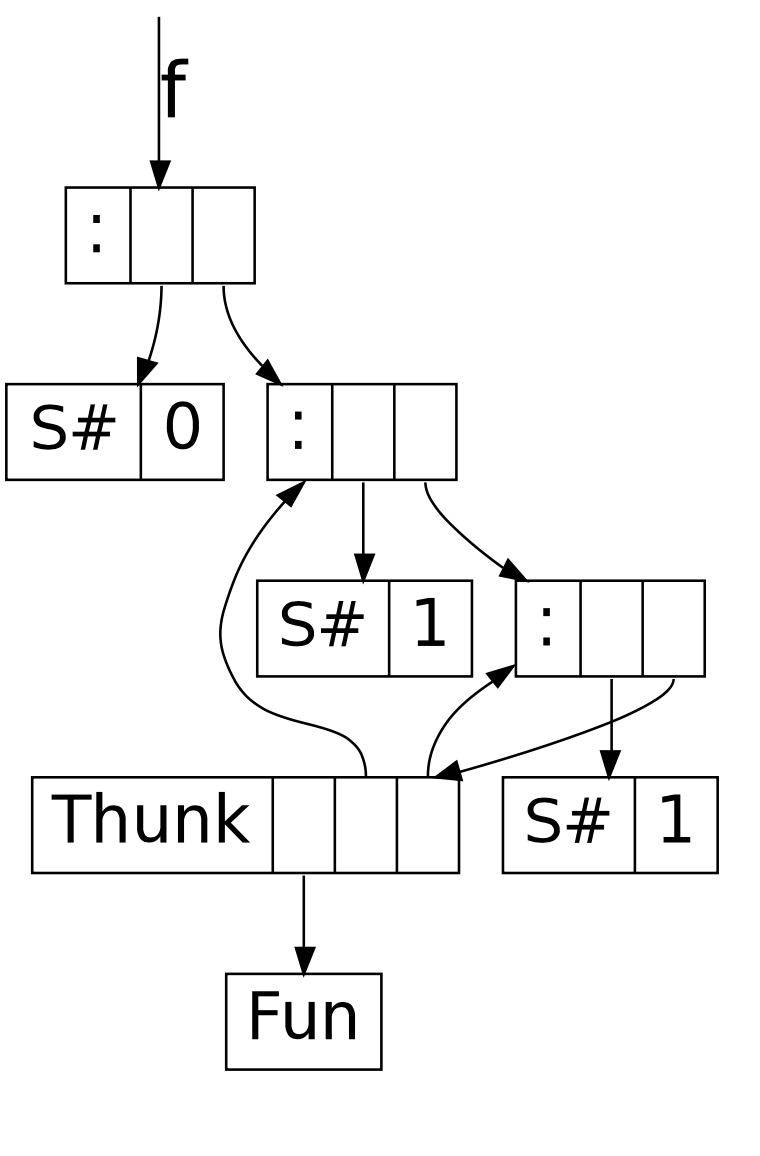
\includegraphics[width = 5cm]{fib2}
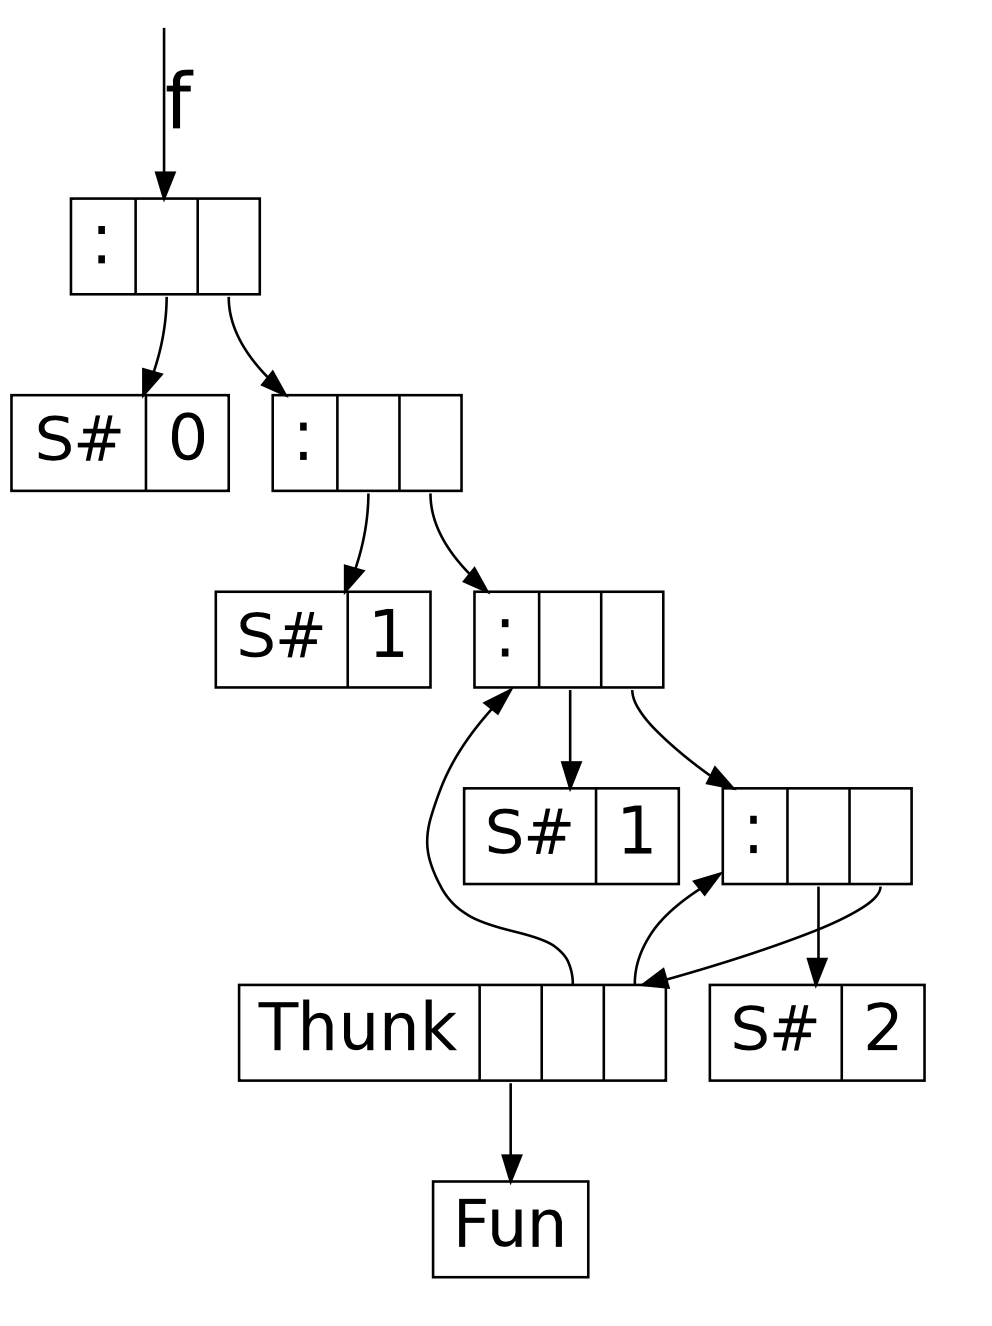
\includegraphics[width = 5cm]{fib3}
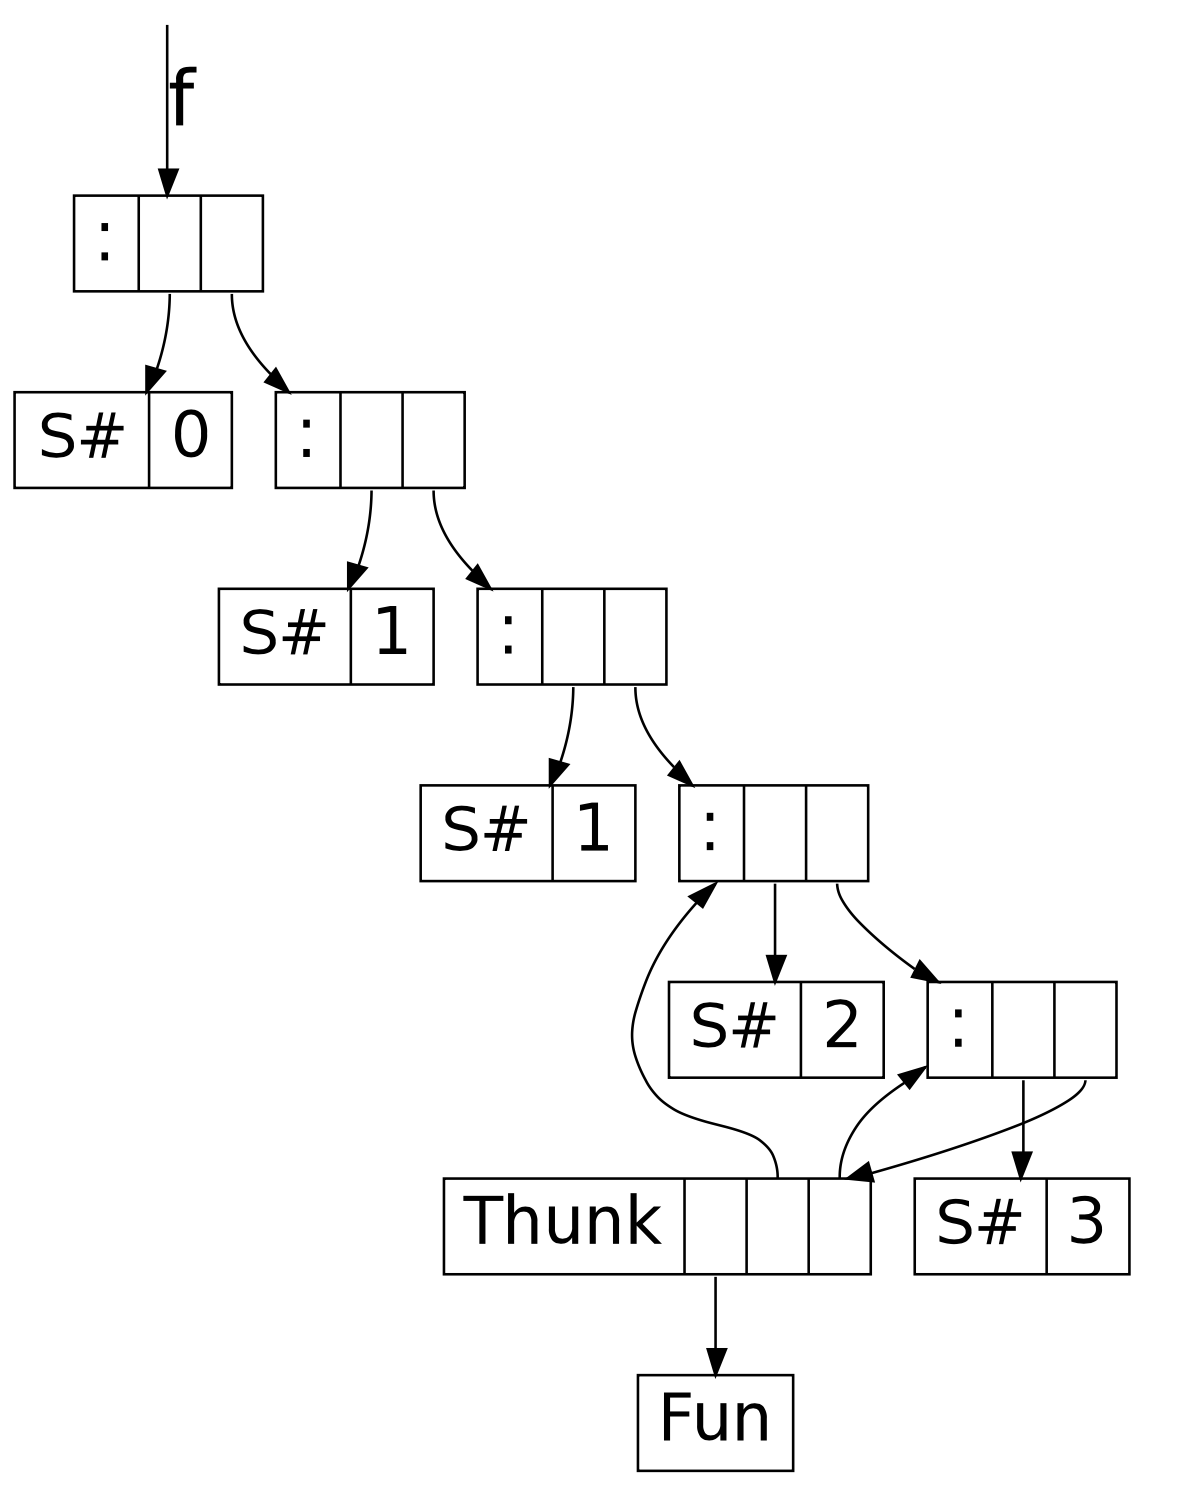
\includegraphics[width = 5cm]{fib4}
\caption{Sample visualizations from the documentation website for ghc-vis\cite{ghc-vis}}
\end{figure}

In the figures above, the leftmost figure corresponds to the state of \texttt{f} after evaluating the \texttt{f !! 2}. The middle figure corresponds to the state of \texttt{f} after evaluating the \texttt{f !! 3} and the rightmost figure corresponds to the state of \texttt{f} after evaluating the \texttt{f !! 4}. In all the above figures, "S\# 1" stands for the Integer data constructor. 

From the above figures, it is easy to see that \texttt{f} is only evaluated in Haskell when required. Any un-evaluated values are \textit{thunked} for future use. The \texttt{Thunk} value contains arrows pointing towards the values that are already calculated, which makes it easy to see and understand the concept of sharing in Haskell.

For the 100\% level we will employ Haskell's lazy evaluation semantics in our visualizations. This will allow the user to interact with the \texttt{Thunk} values in our call tree inside the ghc-vis window. The FWAE parse tree would look similar except it would not be interactive for the lack of \texttt{Thunk} values

If we are not able to make ghc-vis work, we will be trying a different approach. This approach would include looking into Haskell default libraries to create trees and then pretty printing those trees to create the final visualizations.

\begin{thebibliography}{99}

\bibitem{inclass6}
  CPSC 311 2018 WT1 staff.
  (2018).
  An interpreter with first-class functions via environments.
  In \textit{CPSC 311 Definition of Programming Languages: "Lambda Bound"}.
  \url{https://www.ugrad.cs.ubc.ca/~cs311/current/notes/in-class-06.rkt}.

\bibitem{monadic-parsing}
  Graham Hutton, Erik Meijer.
  (1994).
  Monadic Parsing in Haskell.
  \textit{Journal of Functional Programming}, 8(4).
  doi:10.1017/S0956796898003050.
  \url{http://www.cs.nott.ac.uk/~pszgmh/pearl.pdf}.
 
\bibitem{lexical-analysis}
  Wikipedia contributors.
  (2018, October 7).
  Lexical analysis.
  In \textit{Wikipedia, The Free Encyclopedia}.
  Retrieved 20:40, November 4, 2018, from \url{https://en.wikipedia.org/w/index.php?title=Lexical_analysis&oldid=862914890}.
  
\bibitem{parsec-bug}
  Mark Karpov.
  (2015, April 15).
  A possible bug in Text.Parsec.Token.float.
  In \textit{GitHub}.
  Retrieved 20:40, November 4, 2018, from \url{https://github.com/haskell/parsec/issues/35}.
  
\bibitem{parsec}
  Parsec contributors.
  (2018, August 11).
  haskell/parsec: A monadic parser combinator library.
  In \textit{GitHub}.
  Retrieved 14:15, November 13, 2018, from \url{https://github.com/haskell/parsec}.
  
\bibitem{token}
  Herbert Valerio Riedel.
  (2018, February 4).
  parsec/Token.hs at master $\cdot$ haskell/parsec.
  In \textit{GitHub}.
  Retrieved 20:40, November 4, 2018, from \url{https://github.com/haskell/parsec/blob/master/src/Text/Parsec/Token.hs#L503}.
  
\bibitem{fwae-parser}
  Jonathan Chan, Ryan Chen, Samuel Or, and Megha Singhania.
  (2018, November 9).
  lmrjs/fwae-parser.
  In \textit{GitHub}.
  Retrieved November 9, 2018, from \url{https://github.com/lmrjs/fwae-parser/}.
  
\bibitem{learn-haskell}
  Lipovaca Miran.
  (2011).
  Learn You A Haskell For Great Good!: A Beginner's Guide.
  San Francisco, CA: No Starch Press, Inc.
  \url{https://learnyouahaskell.com/}.
  
\bibitem{ghc-vis}
  Felsing Dennis.
  (2012).
  The Ghc-Vis User Guide
  \url{https://lfelsin9.de/nnis/ghc-vis/#fibonacci_numbers}.
  
  
\end{thebibliography}

\end{document}
